\documentclass{beamer}
\usepackage{amsmath}
\usepackage{amssymb}
\usepackage{graphicx}
\usepackage{booktabs}
\usepackage{multirow}
\usepackage{makecell}


\title[PINNs for derivatives pricing]{Using Physics-Informed Neural Networks for pricing derivative financial contracts under stochastic volatility}
\author{Stanislav Borisov}
\institute[HSE University]{HSE University, Sber}
\date{October 14, 2026}

\usetheme{Madrid}
\usecolortheme{seahorse}

\begin{document}

\frame{\titlepage}

\begin{frame}
\frametitle{Outline}
\tableofcontents
\end{frame}

\section{Theory of the derivatives pricing with PDEs}

\begin{frame}
\frametitle{Using PDEs to price financial instruments}
\begin{itemize}
    \item As was established in \textbf{Fischer Black, Myron Scholes - The Pricing of Options and Corporate Liabilities (1973)}, the fair value of any financial contract can be represented by the following Partial Differential Equation:
    \begin{equation*}
        \frac{\partial V}{\partial \tau}=\frac{1}{2}\sigma^2S^2\frac{\partial^2 V}{\partial S^2}+rS\frac{\partial V}{\partial S}-rV
    \end{equation*}
    \item Note, however, that this is a general expression, and to get a fair price of particular derivative, one must apply specific initial and boundary conditions, and sometimes modify the expression to also include Linear Complementarity Problem.
\end{itemize}
\end{frame}

\begin{frame}
\frametitle{Solving Black-Scholes PDE}
\begin{itemize}
    \item For example, consider a European Call Option. It has  terminal and boundary conditions:
        \begin{align*}
            V(0, S) &= \max\{S-K, 0\} \\
            V(\tau, S\to\infty) &= S - Ke^{-r\tau} \\
            V(\tau, S\to0) &= 0
        \end{align*}
    \item This problem can be solved analytically, and it yields famous Black-Scholes Formula:
        \begin{align*}
            C(S, \tau) &= S \, N(d_1) - K e^{-r\tau} \, N(d_2) \\
            d_1 &= \frac{\ln\!\left(S/K\right) + \left(r + \sigma^2/2\right)(\tau)}{\sigma \sqrt{\tau}} \\
            d_2 &= d_1 - \sigma \sqrt{\tau}
        \end{align*}
\end{itemize}
\end{frame}

\begin{frame}
\frametitle{Stochastic volatility}
\begin{itemize}
    \item In reality, however, Black-Scholes model is too basic to reflect the market conditions accurately. Main problem - so called "volatility smile", that BS does not allow.
    \item One of the ways to account for that empirical effect - stochastic volatility (volatility of the price process is its own stochastic process). Today we will look at two popular stochastic volatility models. The first is Heston, which has the following PDE:
    \begin{align*}
        \frac{\partial u}{\partial \tau}
= {} & \frac{1}{2} S^{2} v \frac{\partial^{2} u}{\partial S^{2}}
+ \rho \sigma S v \frac{\partial^{2} u}{\partial S \partial v}
+ \frac{1}{2} \sigma^{2} v \frac{\partial^{2} u}{\partial v^{2}} \\
& + r S \frac{\partial u}{\partial S}
+ \kappa (\theta - v) \frac{\partial u}{\partial v}
- r u.
    \end{align*}
    \item As one can see, the problem's dimensionality increases compared to BS.
\end{itemize}
\end{frame}

\begin{frame}
\frametitle{Numerical methods for Pricing PDE}
\begin{itemize}
    \item Call options under Heston have only quasi-analytical solution, and more complex financial instruments under this model cannot be solved analytically.
    \item Two standard approaches for solving such advanced problems are Monte-Carlo simulations and grid-based solvers for PDEs.
    \item Both have major downsides: slow convergence ($\mathcal{O}(1/\sqrt{n})$) for MC, curse of dimensionality for grid-based PDE solvers.
    \item My work is focused on developing and testing new approach for pricing derivatives with special kind of Neural Network.
\end{itemize}
\end{frame}

\section{Physics-Informed Neural Networks}

\begin{frame}
\frametitle{Physics-Informed Neural Networks}
\begin{itemize}
    \item \textbf{M. Raissi, P. Perdikaris, G.E. Karniadakis - Physics-informed neural networks: A deep learning framework for solving forward and inverse problems involving nonlinear partial differential equations (2019)} introduced Physics-Informed Neural Networks (PINNs).
    \item This architecture allows us to train neural networks on physical dependencies and (optionally) empirical data.
\end{itemize}
\end{frame}

\begin{frame}
\frametitle{Problem setup}
\begin{itemize}
    \item Let $V$ be a neural network which models the solution to a particular PDE.
    \item Given PDE of the general form $f\left(t, \mathbf{x}, u, \frac{\partial u}{\partial t}, \nabla u, \nabla^2 u \ldots, \lambda\right) = 0$, the residual of the network $V$ is $$r_V = f\left(t, \mathbf{x}, V, \frac{\partial V}{\partial t}, \nabla V, \nabla^2 V \ldots, \lambda\right)$$
    \item Partial derivatives with respect to model inputs can be obtained via autodiff.
    \item Then, the problem comes down to writing down a reasonable Loss function for the Network to learn.
\end{itemize}
\end{frame}

\begin{frame}
\frametitle{Network learning problem}
\begin{block}{Setting loss function}
        Define the loss function as:
        $$\mathcal{L}_{total}=\mathcal{L}_{pde}+\mathcal{L}_{boundary}+\mathcal{L}_{initial} + \mathcal{L}_{data}^*+ \mathcal{L}_{lcp}^*$$

        Where:
        \begin{itemize}
            \item \textbf{PDE Loss:} The norm of the solution residual. 
            \item \textbf{Boundary Conditions:} The norm of the difference between boundary conditions and predicted values on boundaries.
            \item \textbf{Initial:} The norm of the difference between initial conditions and predicted values on boundaries.
            \item \textbf{Data Loss:} Additionally, we can add the loss which punishes the divergence from the empirical data (if such data is available).
            \item \textbf{Linear Complementarity Problem Loss:} Optimal stopping loss.
        \end{itemize}
    \end{block}
\end{frame}

\begin{frame}
\frametitle{The scheme of the learning}
\begin{center}
    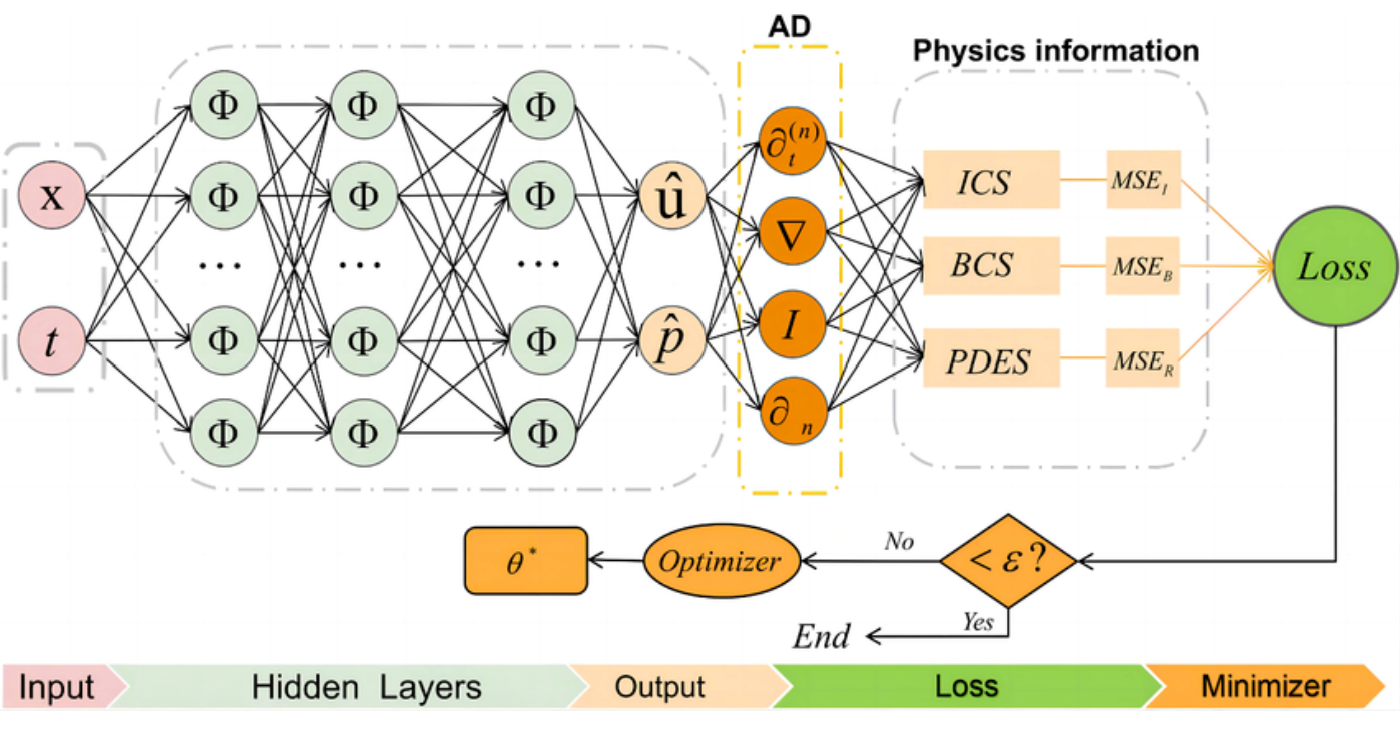
\includegraphics[scale = 0.6]{Graphs/Architecture.png}
\end{center}
\end{frame}

\begin{frame}
\frametitle{Variable transformation}
\begin{itemize}
    \item We can reduce the dimensionality of the problem by transitioning to log-moneyness defined as $x=\log(\frac{S}{K})$ and $u=\frac{V}{K}$. Then, the Heston PDE changes to:
    \begin{align*}
        u_{\tau}
-
\frac{1}{2}v\,u_{xx}
-
\left(r-\frac{1}{2}v\right)u_{x}
-
\rho\sigma v\,u_{xv}
-\\-
\frac{1}{2}\sigma^{2}v\,u_{vv}
-
\kappa(\theta-v)\,u_{v}
+ r u
=0
    \end{align*}
    \item 
This also transforms boundary and terminal conditions. For Calls, they become:
\begin{align*}
    \varphi_{\mathrm{call}}(x) &= \max(e^x-1,0), \\
    u_{\mathrm{call}}(x_{\min},\tau,r,\sigma) &\approx 0, \\
u_{\mathrm{call}}(x_{\max},\tau,r,\sigma)
&\approx e^{x_{\max}} - e^{-r\tau}
\end{align*}
\end{itemize} 
\end{frame}

\begin{frame}
    \frametitle{BS baseline + Neural correction}
  We can help the model learn even further: do not learn the full price, learn only a correction \(U\) on top of a closed-form Black-Scholes baseline.

    \begin{align*}
        u(x,v,\tau;\vartheta)
    \;=\;
    u_{\mathrm{BS}}\!\bigl(x,\tau;\,r,\sigma_{\mathrm{eff}}(v,\vartheta,\tau)\bigr)
    \;+\;
    U_\theta(x,v,\tau;\vartheta)
    \end{align*}

  \vspace{0.6em}
  \begin{itemize}
    \item \(u_{\mathrm{BS}}\): analytical BS price
    \item \(U_\theta\): PINN correction for stochastic-vol effects
    \item PDE residual enforced on the \emph{total} price \(u_{\mathrm{BS}}+U_\theta\)
  \end{itemize}

  \vspace{0.4cm}
  \begin{block}{Why it helps}
    Because we "de-scale" the function the Network learns, adjustment $\to0$ OTM and ITM.
  \end{block}
\end{frame}

\section{Practical results: Heston}
\begin{frame}
\frametitle{Comparison with current pricing methods}
\begin{itemize}
    \item Such alterations to the original equation lead to significant performance boost
    (Heston, errors in normalized price \(u=V/K\), vs.\ COS):
\end{itemize}
    \begin{table}[t]
\centering
\caption{Accuracy and runtime for parametric Heston pricing.}
\label{tab:pricing-comparison}
\begin{tabular}{lcccc}
\hline
Method & RMSE & Max err. & Train & Inf. time \\
\hline
PINN & 0.002 & 0.003 & 9494 s & 151 $\mu$s \\
FD   & 0.002 & 0.005 & [n/a] & $1.5\times 10^{7}$ $\mu$s \\
MC   & 0.006 & 0.011 & [n/a] & 21000 $\mu$s \\
\hline
\end{tabular}
\end{table}
\begin{itemize}
    \item PINNs have high up-front costs, but really fast evaluation speeds once trained. Hence, PINNs are preferred when frequent evaluations of large portfolios of deals are required.
\end{itemize}
\end{frame}

\begin{frame}
\frametitle{Qualitative results - Theta ($\partial V/\partial \tau$)}
    \begin{center}
        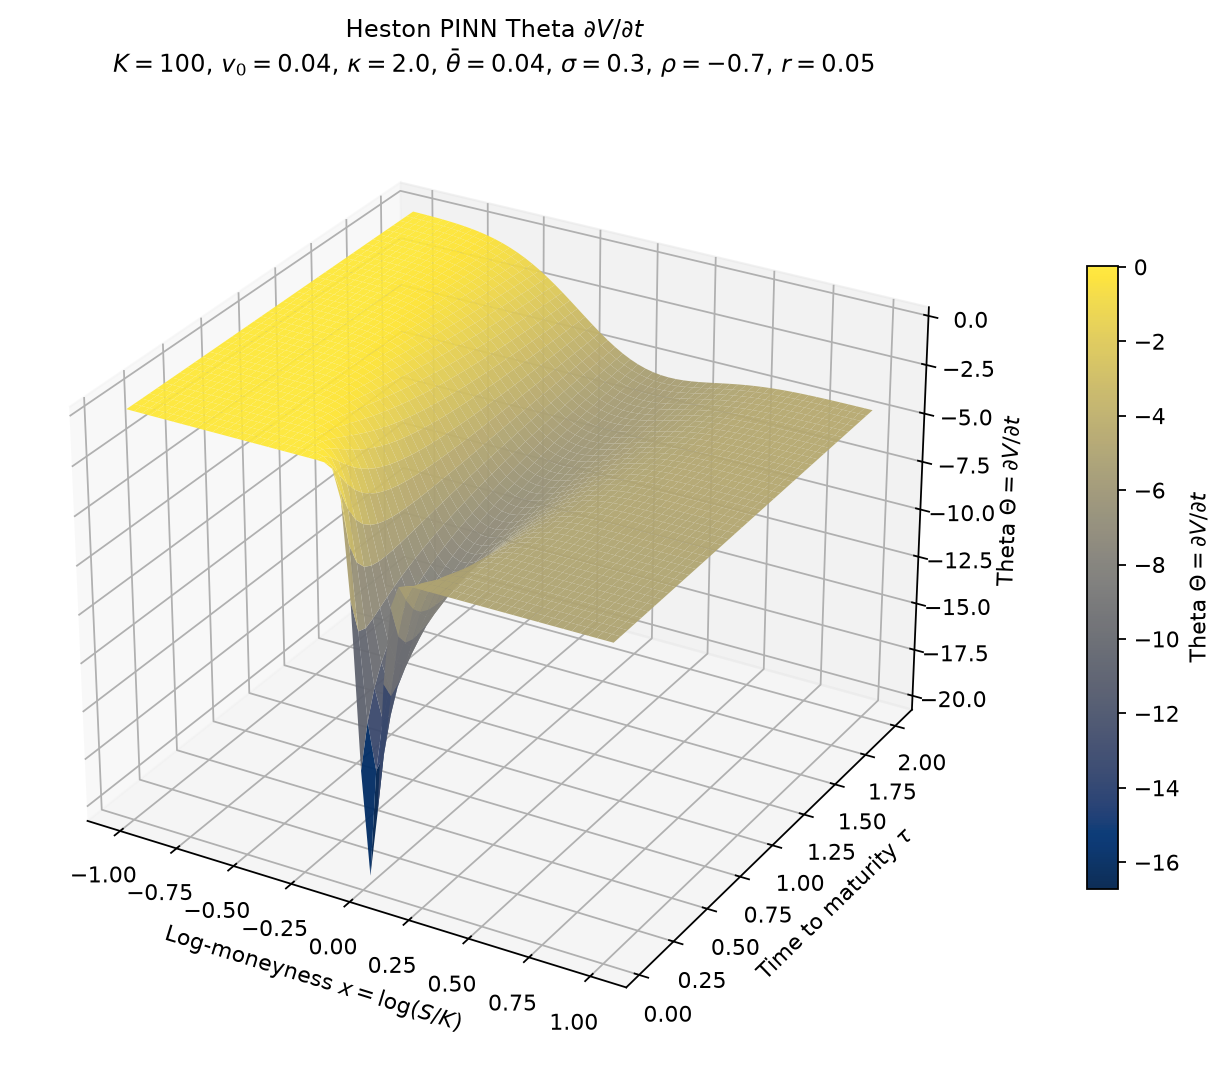
\includegraphics[width=0.7\textwidth]{Graphs/Theta.png}
    \end{center}
\end{frame}

\begin{frame}
\frametitle{Qualitative results - Gamma ($\partial^2 V/\partial S^2$)}
    \begin{center}
        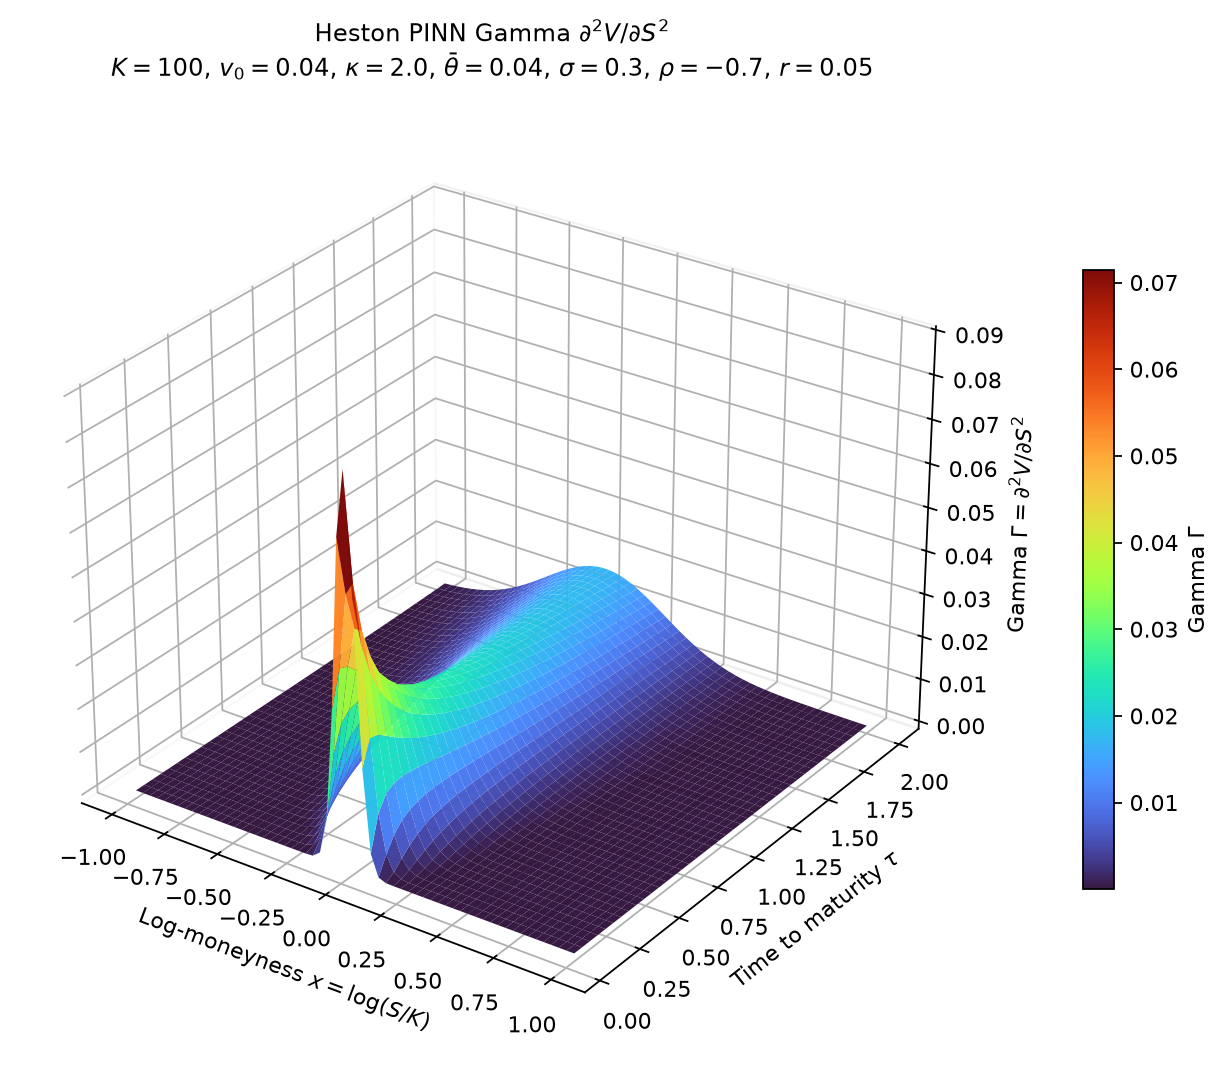
\includegraphics[width=0.7\textwidth]{Graphs/Gamma.png}
    \end{center}
\end{frame}

\section{Practical results: Bergomi}

\begin{frame}
\frametitle{Why do we need more complicated models?}
\begin{center}
    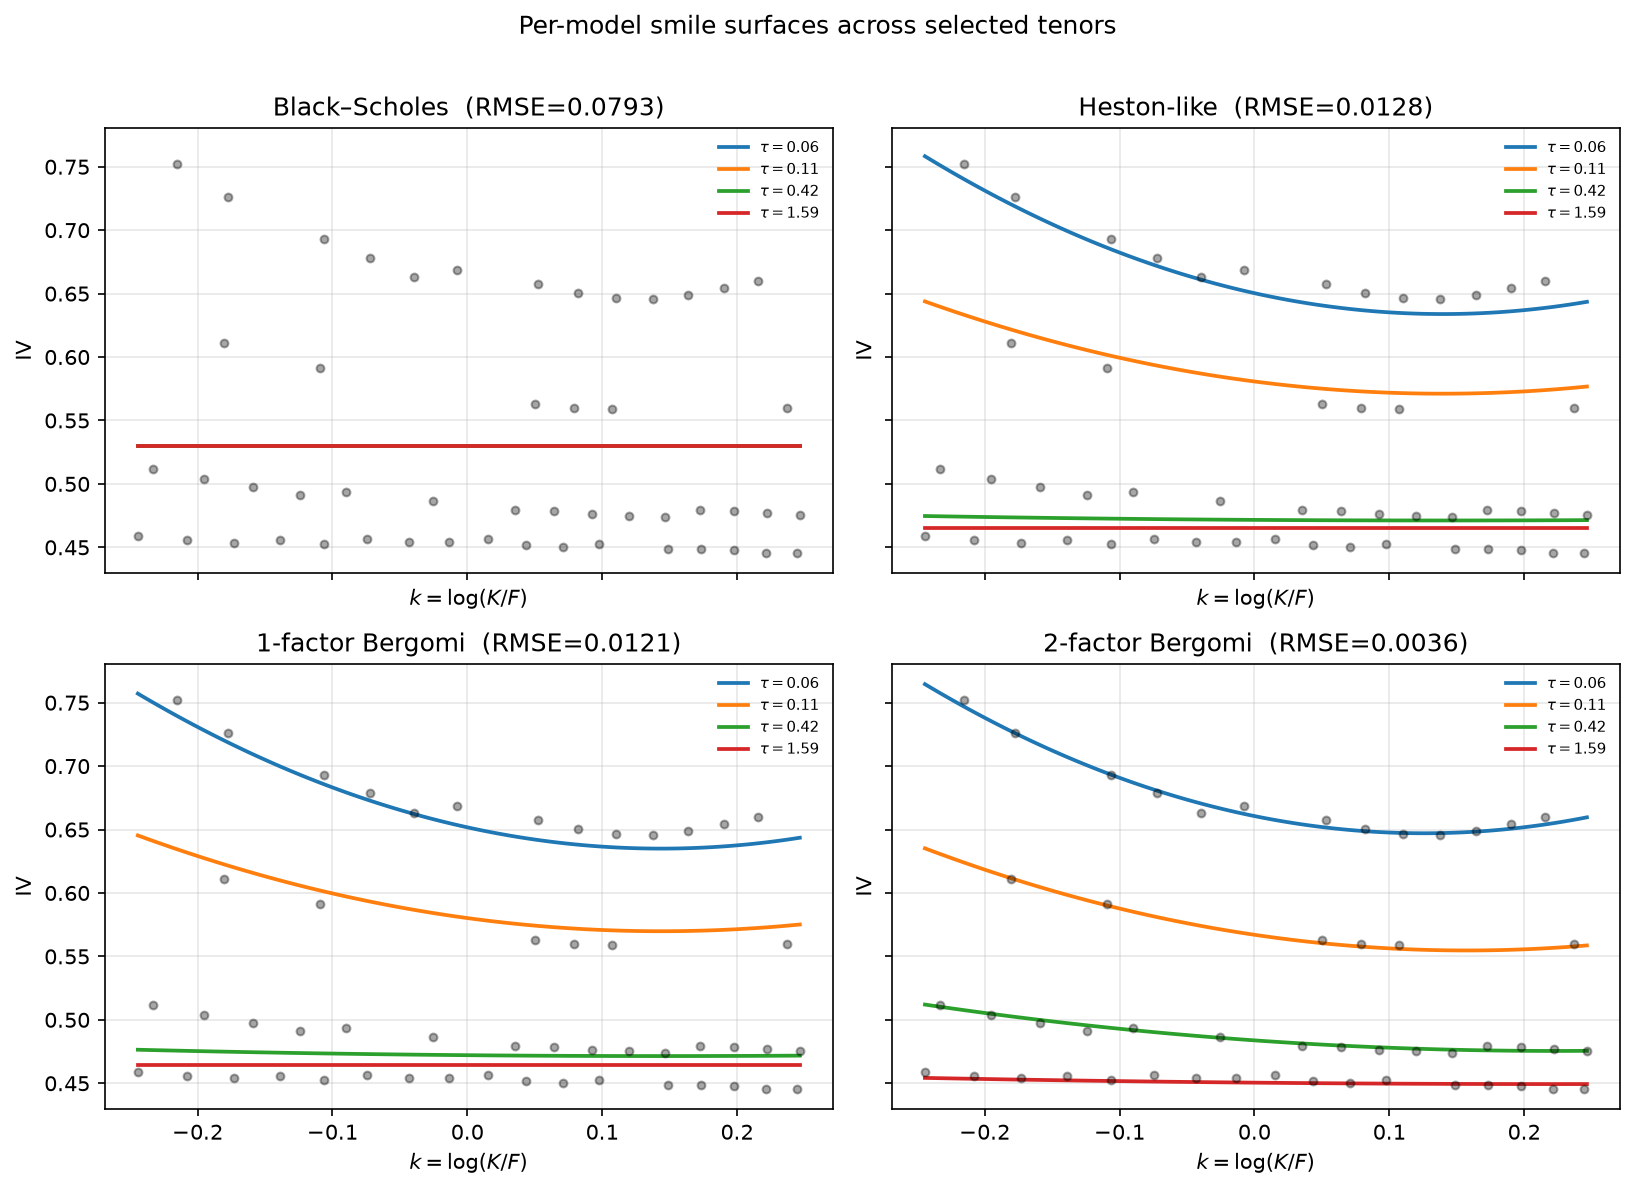
\includegraphics[width=0.88\textwidth]{Graphs/model_surfaces_by_tenor.png}
\end{center}
\end{frame}

\begin{frame}
\frametitle{Why do we need more complicated models?}
\begin{itemize}
    \item Same live equity surface (NVDA): BS is flat; Heston / 1-factor Bergomi improve the short smile but share \emph{one} mean-reversion clock, so long tenors stay compressed.
    \item 2-factor Bergomi adds fast + slow OU factors and fits every tenor cluster.
\end{itemize}
\begin{table}[t]
\centering
\begin{tabular}{lc}
\hline
Model & IV RMSE \\
\hline
Black--Scholes & 0.079 \\
Heston-like & 0.013 \\
1-factor Bergomi & 0.012 \\
2-factor Bergomi & \textbf{0.0036} \\
\hline
\end{tabular}
\end{table}
\begin{itemize}
    \item That gap is the modelling argument for taking the PINN stack beyond Heston.
\end{itemize}
\end{frame}

\begin{frame}
\frametitle{1-factor Bergomi dynamics}
\begin{itemize}
    \item Forward variance is driven by a single OU factor $X$:
    \begin{align*}
        \frac{dS}{S} &= r\,dt + \sqrt{v}\,dW^S, \qquad
        dX = -\kappa X\,dt + dW^X, \\
        v(X) &= \xi_0\exp\!\Bigl(\omega X - \tfrac{\omega^2}{4\kappa}\Bigr)
        \quad\text{(stationary, flat $\xi_0$)}.
    \end{align*}
    \item Pricing PDE in log-moneyness $x=\log(S/K)$, $u=V/K$:
    \begin{align*}
        -u_\tau + (r-\tfrac12 v)u_x + \tfrac12 v\,u_{xx}
        - \kappa X\,u_X + \tfrac12 u_{XX}
        + \rho\sqrt{v}\,u_{xX} - r u &= 0.
    \end{align*}
    \item Same BS-baseline idea as Heston: learn only the correction $U$, then enforce positivity.
\end{itemize}
\end{frame}

\begin{frame}
\frametitle{2-factor Bergomi dynamics}
\begin{itemize}
    \item Fast factor $(\omega_1,\kappa_1,\rho_1)$ + slow factor $(\omega_2,\kappa_2,\rho_2)$:
    \begin{align*}
        dX_i &= -\kappa_i X_i\,dt + dW_i,\quad i=1,2, \\
        v &= \xi_0\exp\!\Bigl(
            \omega_1 X_1+\omega_2 X_2
            -\tfrac{\omega_1^2}{4\kappa_1}-\tfrac{\omega_2^2}{4\kappa_2}
            -\tfrac{\omega_1\omega_2\rho_{12}}{\kappa_1+\kappa_2}
        \Bigr).
    \end{align*}
    \item PDE gains cross terms $\rho_{12}u_{X_1X_2}$, $\rho_i\sqrt{v}\,u_{xX_i}$ and two mean-reversion drifts.
    \item Feature map carries both clocks explicitly (28 features): dual OU state, $\mathrm{mr_{fast/slow}}$, log-variance drive, key cross terms.
\end{itemize}
\end{frame}

\begin{frame}
\frametitle{New techniques introduced for Bergomi PINNs}
\begin{block}{Beyond the Heston recipe}
\begin{itemize}
    \item \textbf{Softplus positivity} ($\beta=400$): $u=\mathrm{softplus}_\beta(u_{\mathrm{BS}}+U)$ --- hard floor without killing ATM gradients.
    \item \textbf{Relative PDE residual}: divide by $1+|L[u_{\mathrm{BS}}]|$ (+ Huber) so the BS operator floor does not stall learning.
    \item \textbf{Short-$\tau$ collocation bias}: mix uniform $\tau$ with $\mathrm{Beta}(0.5,1.5)$ samples --- short smiles drive most of the residual.
    \item \textbf{Help from small MC samples} (2-factor): precompute a \emph{36-point} MC price grid ($\sim 25$k paths) and add a soft supervised anchor loss
    \[
      \mathcal{L}_{\mathrm{data}}
      =\mathbb{E}\!\left[\Bigl(\frac{\hat u-u^{\mathrm{MC}}}{1+|u^{\mathrm{MC}}|}\Bigr)^2\right],
    \]
    while $\lambda_{\mathrm{pde}}$ anneals $0.35\to 1$. Corrects ATM underpricing left by pure PDE training without a huge labelled set.
\end{itemize}
\end{block}
\end{frame}

\begin{frame}
\frametitle{Quantitative results: 1-factor Bergomi}
\begin{itemize}
    \item Checkpoint \texttt{bergomi.pt}; benchmark = scrambled Sobol \textbf{QMC + antithetic differencing (ADD)}.
    \item Fine grid ($K=100$): absolute price errors
\end{itemize}
\begin{table}[t]
\centering
\begin{tabular}{lcccc}
\hline
 & RMSE & MAE & Max $|$err$|$ & Rel.\ RMSE \\
\hline
PINN vs QMC+ADD & 0.137 & 0.110 & 0.321 & 0.061 \\
\hline
\end{tabular}
\end{table}
\begin{itemize}
    \item Smile stress tests (abs.\ $L^\infty$ vs QMC+ADD): baseline 0.30, strong vol-of-vol 0.51, strong neg.\ skew 0.59, mild fast MR 0.21, slow MR 0.92, near-BS 0.17.
    \item Softplus: \textbf{0} negative prices on the fine grid (min $V\approx 0.10$).
\end{itemize}
\end{frame}

\begin{frame}
\frametitle{Quantitative results: 2-factor Bergomi}
\begin{itemize}
    \item Checkpoint \texttt{bergomi2.pt}; market $(\xi_0,\omega,\kappa,\rho)$ with fast/slow clocks; MC 40k paths.
    \item Effect of the small MC-anchor grid:
\end{itemize}
\begin{table}[t]
\centering
\begin{tabular}{lcccc}
\hline
Training & RMSE & MAE & Max $|$err$|$ & ATM $T=1$ \\
\hline
PDE only (prior) & $\approx 0.39$ & $\approx 0.32$ & $\approx 0.66$ & 9.88 \\
+ MC anchors & \textbf{0.309} & \textbf{0.255} & \textbf{0.59} & \textbf{10.29} \\
MC reference & --- & --- & --- & $10.11\pm 0.04$ \\
\hline
\end{tabular}
\end{table}
\begin{itemize}
    \item Best selection loss $\approx 4.2\times 10^{-4}$ (epoch 919); architecture hidden$=96$, depth$=4$.
    \item Anchors are sparse ($\sim$ few dozen points) but enough to pin the ATM level while the PDE residual shapes the smile.
\end{itemize}
\end{frame}

\begin{frame}
\frametitle{Qualitative results: 1-factor price errors}
\begin{center}
    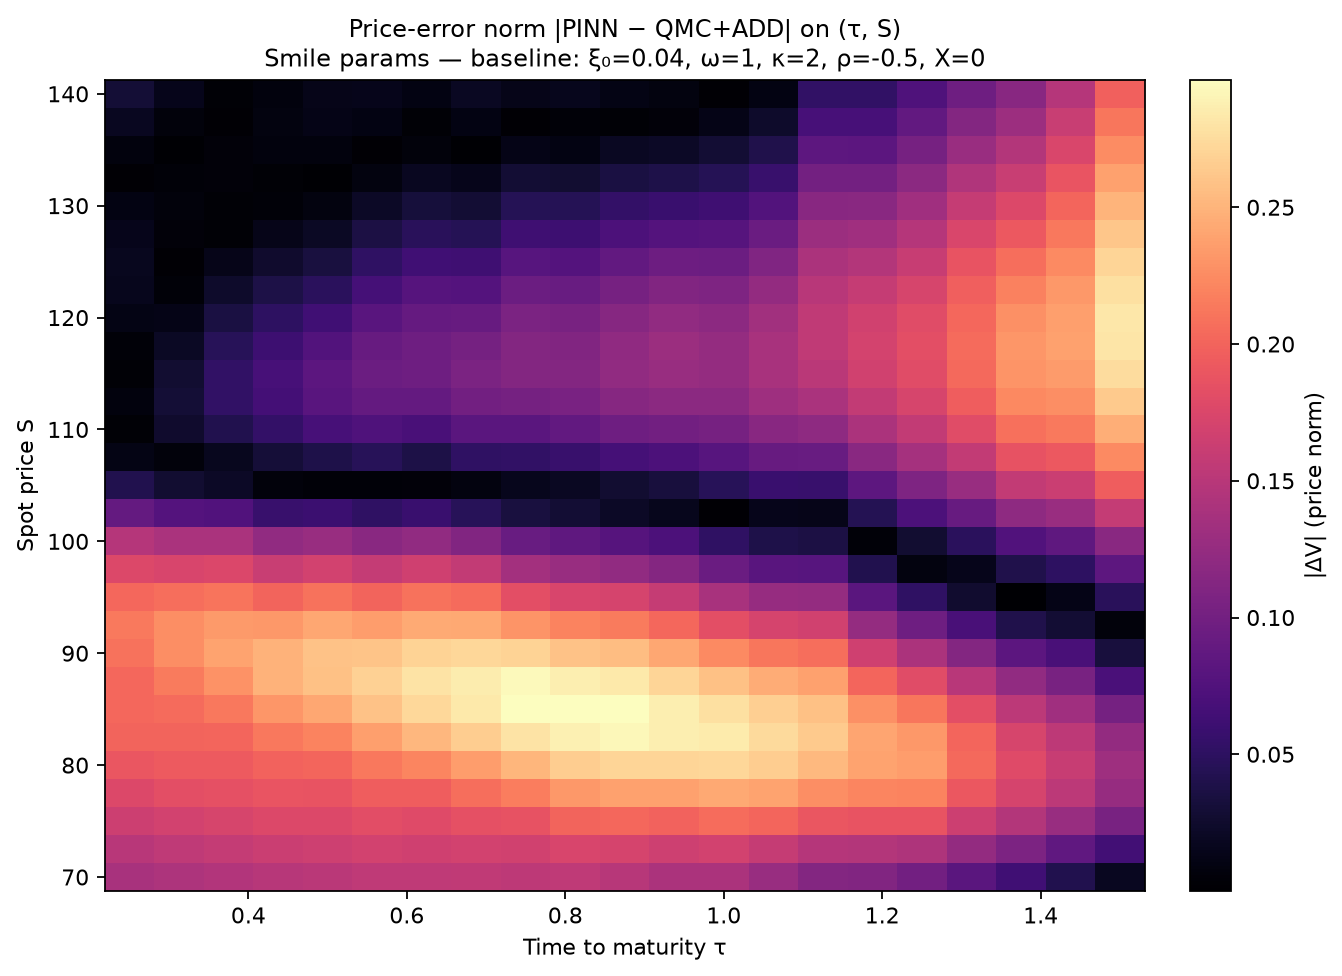
\includegraphics[width=0.72\textwidth]{Graphs/heatmap_baseline.png}
\end{center}
\begin{itemize}
    \item Low-error band near the forward; largest abs.\ errors deep ITM / long $\tau$ --- still sub-dollar on $K=100$.
\end{itemize}
\end{frame}

\begin{frame}
\frametitle{Qualitative results: 2-factor price errors}
\begin{center}
    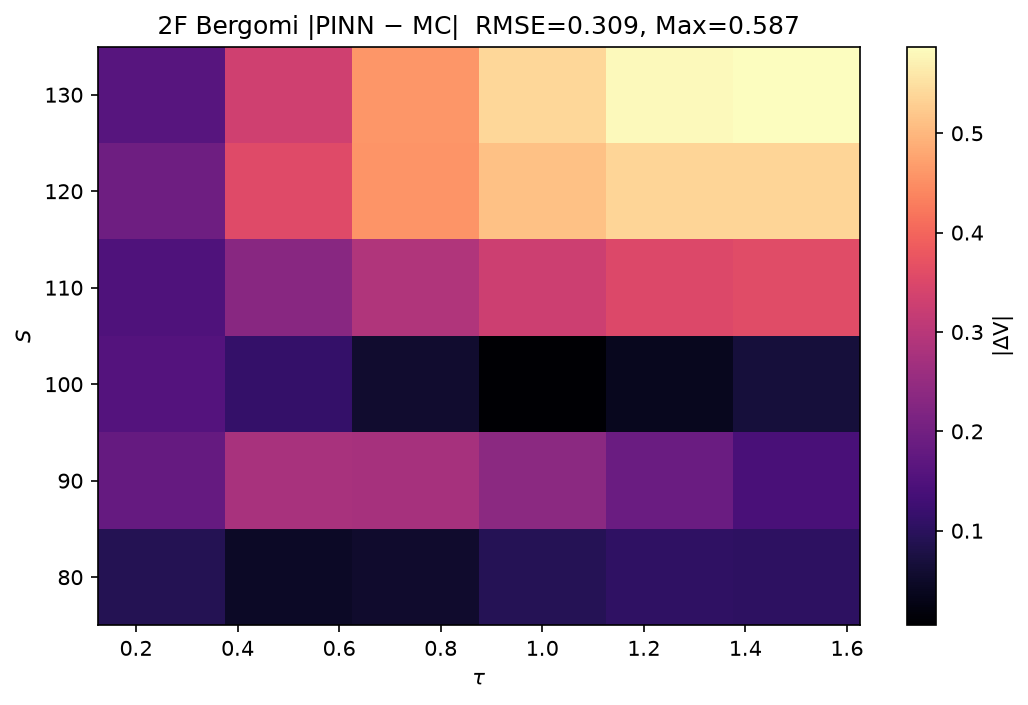
\includegraphics[width=0.78\textwidth]{Graphs/abs_err_heatmap.png}
\end{center}
\begin{itemize}
    \item Errors concentrate at high $S$ and long $\tau$; ATM strip stays dark (anchors + flat-fwd BS baseline).
\end{itemize}
\end{frame}

\begin{frame}
\frametitle{Qualitative: short-dated smile richness}
\begin{center}
    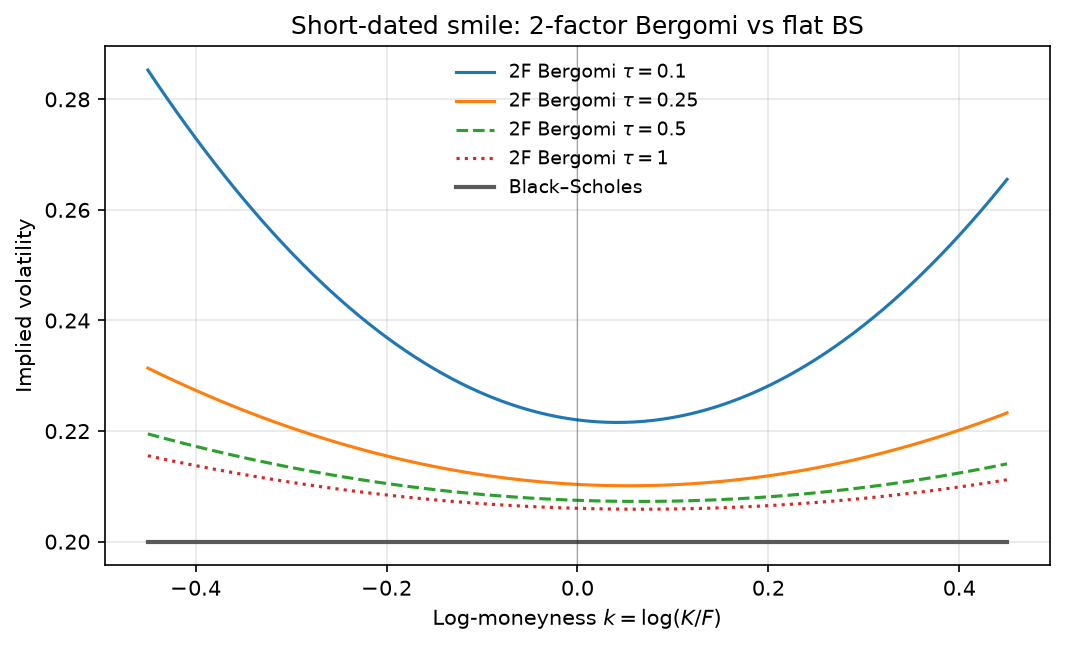
\includegraphics[width=0.82\textwidth]{Graphs/vol_smile_bergomi2_short.png}
\end{center}
\begin{itemize}
    \item 2-factor Bergomi produces a U-shaped short smile that flattens with maturity --- flat BS cannot.
\end{itemize}
\end{frame}

\section{Conclusion and extensions}

\begin{frame}
\frametitle{Advantages of PINNs}
This approach unlocks multiple possibilities for making financial markets more efficient.
\begin{itemize}
    \item With quick pricing, real-time re-evaluation of even large portfolios of derivatives under advanced models is possible. This opens new opportunities for their risk management.
    \item PINNs make the trading of even most complex products accessible to smaller financial institutions (as trained models do not consume lots of compute).
\end{itemize}
\end{frame}

\begin{frame}
\frametitle{Further work}
There is a number of ways I can extend my current research:
\begin{itemize}
    \item Using PINNs to solve inverse problem: given observable market prices, calibrate the parameters of the model.
    \item Applying PINNs to more complex products, which have no analytical pricing.
\end{itemize}
\end{frame}

\begin{frame}
\frametitle{Conclusion}
\begin{center}
    Thank you!

    I am ready to answer any of your questions.
\end{center}
\end{frame}

\end{document}

